% Geometry setup
\documentclass[14pt,a4paper]{article}
\usepackage[margin=1.5cm]{geometry}

% Language setup
\usepackage[T1]{fontenc} % Output character encoding
\usepackage[utf8]{inputenc} % Input character encoding

% Spacing setup
\setlength{\parindent}{0pt} % No paragraph indenting
\setlength{\parskip}{5pt} % Set spacing between paragraphs
\frenchspacing
\newcommand{\rmspace}{\vspace{-19pt}}

% Dependency setup
\usepackage{amsmath}
\usepackage{amssymb}
\usepackage{listings}
\usepackage{float}
\usepackage{graphicx}
\usepackage{hyperref}
\usepackage{url}
\usepackage[comma,authoryear]{natbib}
\usepackage[shortlabels]{enumitem}

% Code pretty print
\usepackage{minted}

% Hyperlink format
\usepackage{xcolor}
\hypersetup{
    colorlinks,
    linkcolor={red!50!black},
    citecolor={blue!50!black},
    urlcolor={blue!80!black}
}

% Title setup
\title{Practice Session Notes: Theory of Algorithms}
\author{Viktória Nemkin (nemkin@cs.bme.hu)}
\date{}

% Custom commands
\newcommand{\lineparagraph}[1]{\paragraph{#1}\mbox{}\\}

% Document
\begin{document}
\maketitle

These are my practice session notes for the Wednesday 16:15 - 18:00 sessions. \textbf{Mistakes are possible}, if you spot any, please contact me at nemkin@cs.bme.hu or in MS Teams.

\section{First}

\section{Second}

\section{Regular expressions, context-free languages}

\subsection{}
\label{3.1}

\lineparagraph{Exercise}

Let $\Sigma = \{a,b\}$ and let language $L$ consist of words
that contain the same number of $a$'s and $b$'s. Is $L$ regular?

\lineparagraph{Solution}

\textbf{Gut feeling} (This is not yet a proof!)

Not regular.

This language is similar to $a^nb^n$ (studied in the lecture). The
main issue with it will be similar: we would need to remember the difference
of the number of $a$'s and $b$'s we have read in so far and only
accept the word if the difference is $0$ after reading in the entire
word.

For every possible difference, we will need a separate state, however the
difference can be arbitrarily large, while we can only have a finite
number of states using Finite Automata, so it won't be possible
to construct such a machine.

\textbf{Proof}

We will do proof by contradiction:

\begin{itemize}
    \item Let's assume that $L$ is regular.
    \item Then, that means that there exists a Deterministic Finite Automata, that accepts the language $L$.
    \item Let's take one such automata, and name it $M$.
    \item Let's count the number of states in $M$ and name this number $n$.
    \item Now let's list exactly $n+1$ specifically chosen words from the $L$ language: $ab$, $aabb$, $a^3b^3$, $\dots$, $a^{n+1}b^{n+1}$.
    \item Then imagine feeding these $n+1$ words into $M$. For all of them, let $M$ read in the $a$ letters and then stop and take note of which state the word is at the moment, halfway-through the operation.
    \item After reading in $a$, $aa$, $a^3$, $\dots$, $a^{n+1}$, since these are $n+1$ cases, while $M$ only has $n$ states, we can use the \href{https://en.wikipedia.org/wiki/Pigeonhole_principle}{Pigeonhole Principle} and say, that there exists at least two different half-words $a^i$ and $a^j$ $(i\neq{}j)$, for which $M$ arrived at the same state after feeding it these inputs. Let's name this state $S$.
    \item Since $a^ib^i$ is in language $L$, it must be accepted by $M$. This means that when we continue from state $S$ and feed in the $b$'s of the word, the machine must arrive in an accepting state. So there exists a path from state $S$ to an accepting state that is traversed by the input $b^i$.
    \item However, $M$ also arrives in state $S$ when it reads $a^j$. We just noted, that if from $S$ it reads $b^i$ it will arrive in an accept state. If we put these two together, it means that $M$ accepts the word $a^ib^j$, where $i\neq{}j$, which is \textbf{not} in $L$, since it doesn't have the same number of $a$'s and $b$'s.
    \item We stated in the beginning that $M$ is a machine whose language is $L$, however we just found a word that is not in $L$, but accepted by $M$, so this is a contradiction.
\end{itemize}

Notes:

\begin{itemize}
    \item This is symmetric, we could also prove that $M$ accepts $a^ib^j$, for $i\neq{}j$ which is also a contradiction, since that word is also not in $L$.
    \item To put it shortly: the machine cannot distinguish $a^i$ and $a^j$ $(i\neq{}j)$ and since $a^ib^i$ and $a^jb^j$ are accepted, so are $a^ib^j$ and $a^jb^i$, which are not in $L$, which is a contradiction.
    \item Note, that this proof is exactly the same as the proof for language $a^nb^n$ studied in the lecture. This is due to the fact, that these languages are similar, for both of them the issue is keeping track of the number of $a$'s to (eventually or simultaneously) compare them to the number of $b$'s.
    \item It is \textbf{not true}, that ''the proof works because $a^nb^n$ is a subset of $L$''. For example, $a^nb^n$ is also a subset of $\Sigma^*$, which is regular!
\end{itemize}

\subsection{Session 3, Exercise 2}

\lineparagraph{Exercise}

Let $\Sigma = \{(,)\}$. Prove that the language of properly matched parentheses sequences is not regular.

\lineparagraph{Solution}

Quite similar to \ref{3f1}. The $n+1$ words from $L$, the language of properly matched parentheses to be used are $()$, $(())$, $(^3)^3$, $\dots$, $(^{(n+1)})^{(n+1)}$, so just substitute $a = ($ and $b = )$.
\subsection{Session 3, Exercise 3}

\lineparagraph{Exercise}

Is the language regular, that consists of sequences of $0$'s of a length that is...
\begin{enumerate}[a.)]
\item an even number?
\item an odd number?
\item a perfect square?
\item a power of $2$?
\end{enumerate}

\lineparagraph{Solution}

\subsubsection{Even number of $0$'s}

Regular.

\textbf{Proof 1}: The regular expression $(00)^*$ matches them.

Proof that this regular expression matches the language:

\begin{itemize}
    \item The $^*$ operator allows any number of repeats, even 0.
    \item Inside the $^*$ operator we have two $0$'s, which can be repeated any number of times to match any even number of $0$'s.
    \item The empty string, also known as zero number of $0$'s contains an even number of $0$'s, so it is part of the language. $(00)^*$ matches the empty string, which is correct.
\end{itemize}

\textbf{Proof 2}: The following DFA accepts the language:

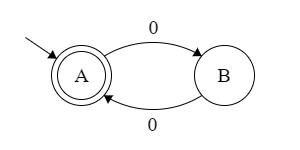
\includegraphics[width=150px]{03/even_zeroes.png}

Proof that this automaton accepts the language:

\begin{itemize}
    \item Words that end up in state $A$ are the words that contain an even number of $0$'s, while words that end up in state $B$ contain an odd number of $0$'s.
    \item The empty string is correctly accepted.
    \item From state $A$, reading another $0$ moves to state $B$, so after reading an even number of $0$'s, if we read one more, now we have an odd number of $0$'s.
    \item And similarly for state $B$.
\end{itemize}

\subsubsection{Odd number of $0$'s}

Regular.

\textbf{Proof 1}: The regular expression $0(00)^*$ matches them.

Proof that this regular expression matches the language:

\begin{itemize}
    \item We have just seen that $(00)^*$ matches an even number of $0$'s.
    \item Adding the $0$ at the front will then match an odd number of $0$'s.
\end{itemize}

\textbf{Proof 2}: The following DFA accepts the language:

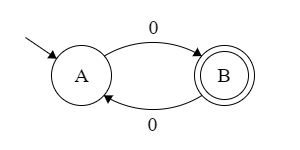
\includegraphics[width=150px]{03/odd_zeroes.png}

Proof that this automaton accepts the language:

\begin{itemize}
    \item This is the same automaton as in the previous exercise, but now the accept state is $B$, to accept an odd number of $0$'s.
\end{itemize}

\subsubsection{A perfect square number of $0$'s}

\textbf{Gut feeling} (This is not yet proof!)

Not regular.

The issue here is going to be, that the length of the accepted words get further and further away from each other as the length of the words increases. We always need to keep track of how far away we are from the next accepted word, how many more $0$'s we need to finally accept. We would need separate states for each of these "$x$ number of $0$'s before we can accept", however $x$ could be arbitrarily large and we only have a finite number of states.

\textbf{Proof}

 Quite similar to \ref{3.1}, the $n+1$ words to use here are of the length of the first $n+1$ square numbers: $0 = 0^{1^2}$, $0000 = 0^{2^2}$, $0^9 = 0^{3^2}$, $0^{16} = 0^{4^2}$, $0^{5^2}$, $0^{6^2}$, $\dots$, $0^{(n+1)^2}$.
 
Then, the finishing of \ref{3.1} is a bit different:

When we find that for an $i\neq{}j$, both $0^{i^2}$ and $0^{j^2}$ end up in the same state $S$, the reasoning is a bit different. Without loss of generality, we can assume that $i<j$. If we were to continue $0^{i^2}$ from state $S$ with $2i+1$ more $0$'s, then the whole input would be $0^{i^2+2i+1} = 0^{(i+1)^2}$, which means that we should accept this word, so from state $S$, for $2i+1$ number of $0$'s we must reach an accept state.

However, this also means that when we continue $0^{j^2}$ (which remember, also arrives in $S$) with $2i+1$ $0$'s, so the word is $0^{j^2+2i+1}$, we will also arrive at the same accept state.

However $j^2+2i+1$ is not a square number. It is between two consecutive square numbers $j^2$ and $(j+1)^2 = j^2+2j+1$, but not equal to either of them:
\begin{itemize}
    \item $j^2 < j^2 + 2i + 1$, since $0<i$.
    \item $j^2 + 2i + 1 < j^2 + 2j + 1$, since $i<j$.
\end{itemize}

Thus, we found a word accepted by $M$, however not in $L$, which is a contradiction.

\subsubsection{A power of $2$}

\textbf{Gut feeling} (This is not yet proof!)

Not regular, the situation is even worse than for square numbers, since powers of $2$ are even further spaced apart as the exponent continues to grow.

\textbf{Proof}

The $n+1$ words to be used are $0^{2^1}$, $0^{2^2}$, $0^{2^3}$, $\dots$, $0^{2^{n+1}}$.

Then similarly to the previous proof, when for $i\neq{}j$, $0^{2^i}$ and $0^{2^j}$ end up in the same state $S$, if we continue by $2^i$ more $0$'s, we should accept, since $0^{2\cdot{}2^i}$ is also a power of two number of $0$'s, however this means  $0^{(2^i + 2^i)}$ will also be accepted, but $2^i + 2^j$ is not a power of $2$, since $i\neq{}j$.
\subsection{Session 3, Exercise 4}

\lineparagraph{Exercise}

Let $\Sigma=\{0,1\}$. Determine the languages of the following regular expressions.

\begin{enumerate}[a.)]
\item $(0+1)^*011(0+1)^*$
\item $1(0+1)^*0$
\item $((0+1)(0+1))^*$
\end{enumerate}

\lineparagraph{Solution}

$(0+1)^*$ is a regular expression that accepts any string from $\Sigma^*$, since $0+1$ accepts either a $0$ or a $1$, and the $^*$ operator allows any number of repeats, including zero.

Thus, $(0+1)^*011(0+1)^*$ is a regular expression that accepts strings that can begin anyhow (including the empty string), then contain the word $011$, then end anyhow, including the empty string. Or, simply put, it accepts all words that contain the string $011$.

For $1(0+1)^*0$, the string must begin with a $1$ and must end with a $0$, while anything, including the empty string can be in between. So this regular expression accepts words that begin with a $1$ and end with a $0$.

For $((0+1)(0+1))^*$, the inner regular expression $(0+1)(0+1)$ accepts any strings with a length of two. Using the $^*$ operator on this allows this to repeat any number of times, allowing for any even length to be accepted, including the length of $0$, which is the empty string.
\subsection{Session 3, Exercise 5}

\lineparagraph{Exercise}

Give regular expressions for the languages over alphabet $\{0,1\}$ that consist of the following words.

\begin{enumerate}[(a)]
\item Words of odd lengths.
\item Words of even length that start and end with $1$.
\item Words containing at least three $0$'s.
\item Words containing an even number of $0$'s.
\item Words of odd lengths starting with $0$ and words of even length starting with $1$.
\item Words of odd length containing subword $00$.
\end{enumerate}

\lineparagraph{Solution}

\subsubsection{Words of odd lengths}

From the previous exercise we know, that $((0+1)(0+1))^*$ accepts the words of even lengths. If we add a $(0+1)$ at the beginning it will add one more character to the lengths, making them odd: $(0+1)((0+1)(0+1))^*$.

\subsubsection{Words of even length that start and end with 1}

To start and end with $1$'s, the regular expression will be $1\text{<something here>}1$. For <something here>, we need to add a regular expression, that together with the two other $1$'s will allow for an even number of characters. So without the two $1$'s, we need an even number of characters, for which we know the regular expression: $((0+1)(0+1))^*$. Putting these together we arrive at $1((0+1)(0+1))^*1$. Since $((0+1)(0+1))^*$ accepts the empty string, the final regular expression will also accept $11$, which is the shortest possible string in the language.

\subsubsection{Words of odd length that start and end with 1}

This was not in the exercise, however I would like to illustrate a point here.

Let's follow the same pattern of thought, as in the previous exercise:
\begin{itemize}
    \item To start and end with $1$'s, the regular expression will be $1\text{<something here>}1$. \item For <something here>, we need to add a regular expression, that together with the two other $1$'s will allow for an odd number of characters.
    \item So without the two $1$'s, we need an odd number of characters, for which we know the regular expression: $(0+1)((0+1)(0+1))^*$.
    \item Putting these together we arrive at $1(0+1)((0+1)(0+1))^*1$.
    \item We have made a mistake...
\end{itemize}

What is the shortest word in this language? It's $1$, which is not accepted by the regular expression above. The issue is that we did not think about the fact, that both starting and ending in a $1$ can also literally mean the same $1$ character, nothing more.

In general, it is always important when building regular expressions from multiple parts, to check for short strings in the language, to see if our expression works for the simplest cases as well.

In this example, to fix the regular expression above, we simply append the missing case at the end: $1(0+1)((0+1)(0+1))^*1 + 1$. This accepts words of length $1$, $3$, and so on, which is what we've wanted.

\subsubsection{Words containing at least three 0's}

Anything can go between the $0$'s, so simply $(0+1)^*0(0+1)^*0(0+1)^*0(0+1)^*$. The three $0$'s between the $(0+1)^*$'s enforce that the string must contain at least three $0$'s.

\subsubsection{Words containing an even number of 0's}

Let's start by words containing exactly two $0$'s: $1^*01^*01^*$. Then, to allow an even number of $0$'s, we can use the $^*$ operator on this: $(1^*01^*01^*)^*$. However, this regular expression has one problem: if the number of $0$'s is zero, we are unable to match anything other than the empty string. However, we would like to match $1^*$, so we can fix this, by either simply appending it at the end: $(1^*01^*01^*)^* + 1^*$, or to make it shorter, simply moving the first one outside of the outer $^*$ operator: $1^*(01^*01^*)^*$.

\subsubsection{Words of odd lengths starting with 0 and words of even length starting with 1}

Let's make two regular expressions and combine them with a $+$ at the end.

Words of odd lengths starting with $0$: $0((0+1)(0+1))^*$. $0$ matching literal $0$ at the beginning, then $((0+1)(0+1))^*$, matching the remaining even number of any characters, which in total result in an odd number of characters.

Words of even length starting with $1$: $1(0+1)((0+1)(0+1))^*$. Since the word must start with a $1$, this no longer can be an empty string. The shortest possible words are $10$ and $11$, which are correctly matched, and can be followed by an even number of characters.

Finally, combinging the two: $0((0+1)(0+1))^* + 1(0+1)((0+1)(0+1))^*$, or to make it shorter: $(0 + 1(0+1))((0+1)(0+1))^*$.

\subsubsection{Words of odd length containing subword 00}

$00$ is even length, so it either starts with an odd length string, then $00$, then an even length string or vice versa: $((0+1)(0+1))^*(0+1)00((0+1)(0+1))^* + ((0+1)(0+1))^*00(0+1)((0+1)(0+1))^*$ and we can shorten this a little like this: $((0+1)(0+1))^*((0+1)00+00(0+1))((0+1)(0+1))^*$. Again, paying attention to the shortest words in the language, which are of length three, this one can match those as well.


\subsection{}

Give regular expressions that are shorter than the following ones but give the same languages.

\begin{enumerate}[a.)]
\item $(0+\varepsilon)^*$
\item $((0+\varepsilon)(0+\varepsilon))^*$
\item $(0+1)^*01(0+1)^*+1^*0^*$
\end{enumerate}
\subsection{}

Give a regular expression whose language consists of all words over $\{0,1\}$ without the subword 110.
\subsection{Session 3, Exercise 8}

\lineparagraph{Exercise}

What language is generated by the following grammar?

\begin{align*}
S &\rightarrow A | B\\
A &\rightarrow 0A1 | 01\\
B &\rightarrow 1B0 | 10
\end{align*}

\lineparagraph{Solution}

We make a decision at $S$, whether to continue with variable $A$, or $B$.

$A$ generates with the following producion rule: $A \rightarrow 0A1|01$, which will put the same number of $0$'s at the beginning as the number of $1$'s at the end, using the ''one to the left and one to the right'' method: every single activation of the $A \rightarrow 0A1$ puts one $0$ to the left and one $1$ to the right, making sure their numbers remain equal as we generate the string.

The empty string is not generated, because there is no production rule that would allow $A$ to terminate in a $\varepsilon$. This is the same as $0^n1^n$, where $n>0$: $L_A=\{0^n1^n|n>0\}$.

With similar logic, $L_B=\{1^n0^n|n>0\}$.

And finally, then $L = L_A \cup L_B$.
\subsection{Session 3, Exercise 9}

\lineparagraph{Exercise}

Give CF-grammars for the following regular languages from Exercise 4:

Let $\Sigma=\{0,1\}$.

\begin{enumerate}[a.)]
\item Contains $011$ as a substring: $(0+1)^*011(0+1)^*$
\item Starts with $1$, ends with $0$: $1(0+1)^*0$
\item Is of even length: $((0+1)(0+1))^*$
\end{enumerate}

\lineparagraph{Solutions}

\subsubsection{Contains $011$ as a substring}

Let's make a variable for producting $(0+1)^*$:

\begin{align*}
A &\rightarrow 0A|1A|\varepsilon
\end{align*}

$A$ generates any string from left-to right, using the first rule if the next character is a $0$ and the second rule if the next character is a $1$. When we reach the end of the string, with no more characters left, the third rule is applied and the production is completed.

Using $A$, we can now do

\begin{align*}
S &\rightarrow A011A\\
A &\rightarrow 0A|1A|\varepsilon
\end{align*}

where $S$ creates the required $011$ substring and puts an $A$ at the beginning and at the end $A$ to generate any optional characters.

\subsubsection{Starts with $1$, ends with $0$}

Using the same $A$, and the same logic as before:

\begin{align*}
S &\rightarrow 1A0\\
A &\rightarrow 0A|1A|\varepsilon
\end{align*}

\subsubsection{Is of even length}

Change up the wording a little: We generate a string that consists of two parts, that are of equal length.

Any time we need to generate something of equal length to something (or any numerical relationship between their lengths) the only way it will work, is if we generate them by the ''one (some) to the left and one (some) to the right'' method.

Right now, any characters are allowed, the only thing that matters is that they are of the same length, so we can do:

\begin{align*}
S &\rightarrow 0S0|0S1|1S0|1S1|\varepsilon
\end{align*}

Or some might prefer this form, may be a bit more cleaner:

\begin{align*}
S &\rightarrow TST|\varepsilon\\
T &\rightarrow 0|1
\end{align*}

\subsection{Session 3, Exercise 10}

\lineparagraph{Exercise}

Give CF-grammar for the language of properly matched parentheses sequences.

\lineparagraph{Solution}

Again, apply the ''one to the left, one to the right'' method, and generate the matching pairs of parentheses at the same time!

Starting out with something like this, which is not yet correct:

\begin{align*}
S &\rightarrow (S)|\varepsilon
\end{align*}

However, this only generates $((((\dots))))$, while we can also add properly matched parentheses next to each other:

\begin{align*}
S &\rightarrow SS|(S)|\varepsilon
\end{align*}

Proof that this is correct:

To generate a string of properly matched parentheses, we start by counting the number of the outermost parentheses pairs, and use the first rule to generate an equal number of $S$ variables. Then, we use the second rule once on all of them, to put down the outer parentheses. Then, we repeat for the inner strings, which must be also properly matched parentheses. When there is no more inner string, we use the third rule to terminate the generation.

No improper strings can be generated, since the second rule guarantees that only matched pairs are generated in that step, while the inner string will also be a properly matched parentheses sequence, since it is generated from $S$ as well. The first rule is correct also, since properly matched parentheses can be concatenated to arrive at another properly matched parentheses string.
\subsection{Session 3, Exercise 11}

\lineparagraph{Exercise}

Determine the languages generated by the following grammars.

a.)
\begin{align*}
T &\rightarrow TT | aTb | bTa | a | \varepsilon
\end{align*}

b.)
\begin{align*}
R &\rightarrow TaT\\
T &\rightarrow TT | aTb | bTa | a | \varepsilon
\end{align*}

\lineparagraph{Solution}

a.)
\begin{align*}
T &\rightarrow TT | aTb | bTa | a | \varepsilon
\end{align*}

We can quickly see, that for any word generated by this grammar, the number of $a$'s can not be less than the number of $b$'s in it.

Intuitively we have a gut feeling, that due to the first rule, the order in which these characters appear might be completely arbitrary and actually all words like this can be generated.

We will show that this is true:

\textbf{Proof}

Statement: Any word for which the number of $a$'s is not less than the number of $b$'s can be generated using the production rules above.

We will be using mathematical induction for the length of the generated strings.

For the base case, of length either $1$ or $0$, the word can either be $\varepsilon$ (the empty string) or $a$, both of which can be generated (in one step, using either the fourth or the fifth rule).

Inductive step: We will prove that if the statement is true for any word of length less than $n$, then it is also true for any word of lengfth $n$.

Let's take a word of length $n$: $w = x_1x_2,\dots,x_n$.

Let's take the smallest $i$, for which in the word $w_{1..i}$ there is exactly as many $a$'s as $b$'s.

If there is no such $i$, but we are in the language, the only possible way is that all prefixes contain strictly more $a$'s, then $b$'s, specifically for $i=1$ as well, which means that $w_1 = a$. We can generate this letter by using the first and the fourth production rules as such $T \rightarrow TT \rightarrow aT$, where $T$ would have to generate the word $w_{2..n}$, which is of length $n-1$, which can be generated via $T$ according to the induction hypothesis.

If there is such $i$, then $x_i\neq{}x_1$, since $i$ is the first time the number of $a$'s is equal to the number of $b$'s.

Then, we can use the first, then either the second or the third production rule to generate the characters $x_1$ and $x_i$, such as $T \rightarrow TT \rightarrow x_1Tx_iT$. Where the remainder two parts of the word $w_{2..i-1}$ and $w_{i+1..n}$ are also 
in the language and can be generated using $T$, since their lenght is less than $n$, according to the induction hypothesis.

b.)
\begin{align*}
R &\rightarrow TaT\\
T &\rightarrow TT | aTb | bTa | a | \varepsilon
\end{align*}

$T$ is the same as in a.), and due to $R$, now the number of $a$'s must be strictly greater than the number of $b$'s.
\subsection{Session 3, Exercise 12}

\lineparagraph{Exercises}

Determine the language generated by this grammar.

\begin{align*}
R &\rightarrow XRX | S\\
S &\rightarrow aTb | bTa\\
T &\rightarrow XTX | X | \varepsilon\\
X &\rightarrow a | b
\end{align*}

\lineparagraph{Solution}

Let's get rid of $X$ first:

\begin{align*}
R &\rightarrow aRa | aRb | bRa | bRb | S\\
S &\rightarrow aTb | bTa\\
T &\rightarrow aTa | aTb | bTa | bTb | a | b | \varepsilon\\
\end{align*}

Then $S$:

\begin{align*}
R &\rightarrow aRa | aRb | bRa | bRb | aTb | bTa \\
T &\rightarrow aTa | aTb | bTa | bTb | a | b | \varepsilon\\
\end{align*}

\begin{itemize}
    \item $R$ generates a string to its left and to its right, of the same length using the
''one to the left, one to the right'' method.
    \item Importantly, when it changes into $T$, only two transitions are allowed: where the generated characters are different.
    \item Then, $T$ continues generating a string to its left and to its right, of the same length using the ''one to the left, one to the right'' method.
    \item Then it terminates in either $a$, $b$, or $\varepsilon$.
\end{itemize}

This is the opposite of a palindrome generator: due to that transitioning from $R$ to $T$, there must be at least one position where the palindromness of the string is broken. Other positions can be either matching, or non-matching, but there will be at least one, where the characters don't match.

Proof:

Any non-palindrom can be generated with this: since it is a non-palindrom, there is a position where the mirrored position contains the wrong character. Use the first 4 rules until we reach that position, then use the 5th or the 6th rule to move to $T$, then continue using rules 7 to 10, until we are left with a single character (for a string of odd length), then use rule 11 or 12, or no characters (for a string of even length), then use the last rule.

Any palindrom can not be generated, since there is no way to transition $R$ into a $T$ (no position breaks the palindromness), so the generation can never terminate.




\end{document}
